\section{Entanglement measures}\label{sec:2:entanglement-measures}
Checking whether an arbitrary state $\rho$ is entangled or not is no easy task. In fact, this problem is known to be NP-hard \cite{Gurvits_2003}.
A state $\rho_{AB} \in \mathcal{H}_A\otimes\mathcal{H}_B$ is called entangled, if it is \emph{non-separable}, that is, it cannot be expressed as a tensor product of two subsystems $\rho_A \in \mathcal{H}_A$ and $\rho_B \in \mathcal{H}_B$.
Only for specific cases - like the case of two qubits or qubit-qutrit - a simple sufficient criterion for determining the separability of a general mixed state is known:
The positive partial transpose (PPT) criterion states, that if the partial transpose of the density matrix is positive ($\rho^{\Gamma_A} > 0$ \footnote{A matrix is defined as positive (\q{positive definite}), if all eigenvalues are positive.}), the state $\rho$ is separable \cite{Horodecki_2009,Plenio_2005a}.
In other words, if $\rho^{\Gamma_A}$ has negative eigenvalues, $\rho$ is guaranteed to describe an entangled state.
The inverse is true, if and only if the dimension of $\rho_A\otimes\rho_B$ is $2\times2$ or $3\times2$ \cite{Horodecki_2009} - otherwise, only having non-negative eigenvalues doesn't necessarily result in an unentangled system.
The partial transpose with respect to a subsystem $i$ can be understood in the same way as the partial trace, where the operation (in this case the transform) is performed only on indices corresponding the subsystem $\rho_i$.
It is defined for an arbitrary density operator $\rho = \sum_{ijkl}p^{ij}_{kl}\ketbra{i}{j}\otimes\ketbra{k}{l}$ as $\rho^{\Gamma_A} = \sum_{ijkl}p^{ji}_{kl}\ketbra{i}{j}\otimes\ketbra{k}{l}$.
To see the necessity of the PPT criterion, consider a separable mixed state $\rho$, which can be generally expressed as 
\begin{equation}\label{eq:2:separable-state}
  \rho = \sum p_i \rho_{A}^i\otimes\rho_{B}^i .
\end{equation}
The partial transpose is in this case trivial:
\begin{equation}
  \rho^{\Gamma_A} = \sum p_i (\rho_{A}^i)^T \otimes \rho_{B}^i .
\end{equation}
Since the transpose preserves eigenvalues, the transposed subsystem $A$ is still positive $(\rho_{A}^i)^T > 0$ and describes again a valid quantum state. It follows, that $\rho^{\Gamma_A}$ is positive as well.
If somehow $\rho^{\Gamma_A}$ has any negative eigenvalues, this can only mean that the initial state $\rho$ is not separable and cannot be expressed in the form of eq. \eqref{eq:2:separable-state} and the necessity of the criterion is shown.

For quantifying entanglement in a more precise way, a mathematical quantity called \emph{entanglement measure} can be used. A good measure should be able to capture the essential features of entanglement. One can axiomatically state what properties such a measure $E(\rho)$ should have \cite{Plenio_2005a,Horodecki_2009}:
\begin{description}
  \item[Normalization] An entanglement measure should be a map from a state to a positive real number:
  \begin{equation}
    \rho \rightarrow E(\rho) \in \mathbb{R}^+
  \end{equation}
  where usually the maximally entangled state has $E=1$.
  \item[Monotonicity under LOCC] $E$ should not increase under local operations and classical communications. This is the most important postulate for an entanglement measure and often cited as the \textit{only} required postulate.
  \item[Vanishing on separable states] $E(\rho)=0$ if $\rho$ is separable
  \item[] Often one finds additional properties useful like \textit{convexity} $E(\sum p_i \rho_i) \leq \sum p_i E(\rho_i)$ or (full) \textit{additivity} $E(\rho \otimes \sigma) = E(\rho) + E(\sigma)$.
\end{description}
A function that satisfies these conditions is often called an \textit{entanglement monotone}.

The \emph{negativity} $\mathcal{N}$ is such an entanglement monotone \cite{Vidal_2001,Plenio_2005a} that used the PPT criterion to determine if a state is entangled or not. It is defined as 
\begin{equation}\label{eq:2:negativity}
  \mathcal{N} = \frac{\norm{\rho^{\Gamma_A}}_1 - 1}{2}
\end{equation}
where $\norm{A}_1 = \tr\abs{A} = \tr \sqrt{A^\dagger A}$ is the trace norm. The negativity however is not additive and a more universally applicable and widely used entanglement measure is the \emph{logarithmic negativity} \cite{Plenio_2005}
\begin{equation}\label{eq:2:logarithmic-negativity}
  E_N(\rho) = \log_2\norm{\rho^{\Gamma_A}}_1 .
\end{equation}
The monotonicity of the logarithm implies, that $E_N$ is an entanglement monotone as well.
Furthermore it is noteworthy, that $\norm{\rho^{\Gamma_A}} = \norm{\rho^{\Gamma_B}}$ as will be shown below. Therefore, the logarithmic negativity is symmetric under exchange of to the subsystem.

\begin{proposition}
  a) The partial transpose w.r.t. subsystem $A$ is equal to the transposed partial transpose w.r.t. subsystem $B$: $\rho^{\Gamma_A} = (\rho^{\Gamma_B})^T$. 
  b) The trace norms of partially transposed density operators w.r.t. any subsystem are equal: $\norm{\rho^{\Gamma_A}}_1 = \norm{\rho^{\Gamma_B}}_1$.
\end{proposition}
\begin{proof}
  a) A general density matrix $\rho$ can be expressed as
  \begin{equation*}
    \rho = \sum_{i,j,k,l} \rho_{ij,kl} \ketbra{i}{j}_A\otimes\ketbra{k}{l}_B
  \end{equation*}
  The partial transpose with respect to subsystem $B$ is then defined as 
  \begin{equation*}
    \rho^{\Gamma_B} \equiv \sum_{i,j,k,l} \rho_{ij,kl} \ketbra{i}{j}_A\otimes\left(\ketbra{k}{l}_B\right)^T = \sum_{i,j,k,l} c_{ij,kl} \ketbra{i}{j}_A\otimes\ketbra{l}{k}_B
  \end{equation*}
  The complete transpose of this is
  \begin{equation*}
    (\rho^{\Gamma_B})^T = \sum_{i,j,k,l} \rho_{ij,kl} \left(\ketbra{i}{j}_A\right)^T\otimes\left(\ketbra{l}{k}_B\right)^T = \sum_{i,j,k,l} c_{ij,kl} \ketbra{j}{i}_A\otimes\ketbra{k}{l}_B \equiv \rho^{\Gamma_A}
  \end{equation*}
  b) Clear by a) and by using \cref{lemma:trace-norm-hermitian} and the fact that the eigenvalues of a square matrix $A$ and $A^T$ are equal.
\end{proof}

The logarithmic negativity is very easy to calculate compared to other entanglement measures.
If the eigenvalues of $\rho$ are known, the logarithmic negativity can be directly computed, as will be demonstrated below. Since this thesis focuses on low-dimensional $4 \times 4$ systems, single eigenvalues can be determined with low effort analytically as well as numerically with great stability.

\begin{lemma}\label{lemma:trace-norm-hermitian}
  The trace norm $\norm{A}_1 \equiv \tr \sqrt{A^\dagger A}$ of a hermitian matrix $A$ is equal to the sum of the absolute eigenvalues of $A$.
\end{lemma}
\begin{proof}
  This can be immediately seen by the spectral decomposition $\operatorname{\lambda}(A) = \{\lambda_1,...\}$:
  \begin{equation*}
    \tr \sqrt{A^\dagger A} = \tr \sqrt{A^2} = \tr{U\sqrt{\diag(\lambda_1, \dots)^2}U^\dagger} = \sum_i \sqrt{\lambda_i^2} = \sum_i \abs{\lambda_i}.
  \end{equation*}
\end{proof}

\begin{proposition}\label{proposition:negativity}
  The negativity eq. \eqref{eq:2:negativity} is given as the absolute sum of all negative eigenvalues of $\rho^{\Gamma}$: 
\begin{equation}
    \mathscr{N}(\rho) \equiv \frac{\norm{\rho^{\Gamma}}_1 - 1}{2} = \abs{\sum_{\lambda_i < 0} \lambda_i}.
\end{equation}
\end{proposition}
\begin{proof}
  The proof is in parts given by Vidal and Werner \cite{Vidal_2001}. It is known that the density matrix is hermitian: $\rho = \rho^\dagger$. Using \cref{lemma:trace-norm-hermitian}, the trace norm of the density matrix is is given as $\norm{\rho}_1=\sum \lambda_i = \tr \rho = 1$. The partial transpose $\rho^{\Gamma}$ obviously also satisfies $\tr \rho^{\Gamma} = 1$ but might have negative eigenvalues. Since $\rho^{\Gamma}$ is still hermitian, the trace norm is given by
  \begin{equation*}
    \norm{\rho^{\Gamma}}_1 = \sum_i\abs{\lambda_i} = \sum_{\lambda_i \ge 0} \lambda_i + \sum_{\lambda_i < 0} \abs{\lambda_i} = \sum_i \lambda_i + 2\sum_{\lambda_i < 0} \abs{\lambda_i} = 1 + 2\sum_{\lambda_i < 0} \abs{\lambda_i} ,
  \end{equation*}
  where in the last step $\sum \lambda_i = \tr \rho^{\Gamma} = 1$ was used.
\end{proof}
\begin{remark}
  The PPT criterion states, that if $\rho^{\Gamma}$ has negative eigenvalues, the state $\rho$ is entangled. The negativity uses this criterion for a quantification of entanglement. This motivates the name \textit{negativ}ity.
\end{remark}

Calculating the logarithmic negativity of the evolved state eq. \eqref{eq:2:evolved-state}, it is possible to quantify how the entanglement behaves in time. A straight forward computation following the calculation methods established above yields (for detailed calculations see appendix \ref{apx:E_N-exemplary})
\begin{equation}\label{eq:2:entanglement-dynamics-parallel}
  E_N(\ketbra{\psi(t)}) = \log_2\left(1 + \abs{\sin \Delta\phi}\right) .
\end{equation}
As expected, the states are not entangled for $\Delta\phi = k\pi \ k\in\mathbb{Z}$ and maximum entanglement $E_N = 1$  is reached
for $\Delta\phi = 2\pi k \pm \pi/2$.
This result aligns with the previous observations by
demanding that the evolved state eq. \eqref{eq:2:evolved-state-factored}  is separable.
The complete entanglement dynamics are shown in \cref{fig:2:entanglement-dynamics}.
\begin{figure}[!htbp]
  \centering
  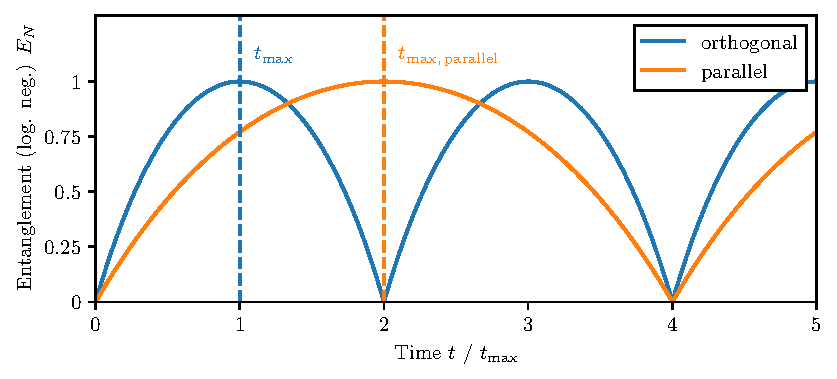
\includegraphics[width=\textwidth]{./../figures/ideal-entanglement/EN-time.pdf}
  \caption{Entanglement dynamics quantified by the logarithmic negativity $E_N$ for two different orientations of the spatial superpositions. The parallel orientation (\textbf{orange}) is shown in \cref{fig:2:simple-problem} and the orthogonal orientation (\textbf{blue}) was taken from Ref. \cite{Pedernales_2023}, where the cat-states are right-angled compared to the parallel configuration. The maximal amount of entanglement is reached after a time given by eq. \eqref{eq:2:t-max-parallel} and for reasonable parameters this equates to $t_\mathrm{max,\,orthogonal} \equiv t_\mathrm{max} \approx 129\si{ms}$.}
  \label{fig:2:entanglement-dynamics}
\end{figure}
Additionally, this figure depicts the entanglement generation in the \q{orthogonal orientation}, where both superpositions are aligned in a straight line right-angled to the previously used setup in \cref{fig:2:simple-problem}.

The time $t_\mathrm{max,\,parallel}$ at which the states are maximally entangled for the first time, can be calculated by using the definition of $\Delta\phi$ from eq. \eqref{eq:2:definition-delta-phi} as
\begin{equation}\label{eq:2:t-max-parallel}
  t_\mathrm{max,\,parallel} = \frac{8 \pi L^3\hbar}{G M_A M_B (\Delta x)^2} .
\end{equation}
In the orthogonal orientation, this point in time is reached twice as fast \cite{Pedernales_2023}. This is because in this orientation, the difference in distances between the cat-states is maximized and consequently the relative dynamical phase build-up is faster compared to the parallel orientation resulting in a faster entanglement rate.

This suggests, that the orthogonal orientation might be beneficial as it requires shorter coherence times. This effect is studied in more detail in \cref{sec:4:optimal-setup}.
To give an estimation of the coherence times needed, consider two identical silica nano-sphere with density $\rho=2648\si{kg/m^3}$ and radius $R=10^{-5}\si{m}=10\si{\mu m}$ separated by a distance $2L = 4R$.
The superposition size is in the order of $100\si{nm}$.
The maximum entanglement in the parallel configuration is reached after a time $t_\mathrm{max,\,parallel} \approx 258\si{ms}$ which is a quite long and challenging experimentally considering that usual in the order of nano-seconds \cite{OConnell_2010}.
